\chapter{Validation}
\label{sec:Validation}

This chapter is dedicated to the validation of the framework on real-world data. In \autoref{ch:FeatureExtraction}, the reference dataset \cite{lee2007bearingdataset} has been introduced. Firstly, the \texttt{python} implementation of the framework is validated on the \gls{ims} dataset several times with different configurations to show the flexibility of the framework, and try to find the best configuration for the dataset. 

The first test in the \gls{ims} dataset is carried out with all the machine learning models developed, then only the K-mean model is used in the following tests. In all tests an outlier filter has been implemented, so that the \gls{mla} will warn about the novelty behavior only if two consecutive snapshots are labeled as outliers. 

Then, the \gls{glo:edge} implementation of the framework is validated experimentally on a machine and with a laboratory shaker.



\maskongoig{
\section{\gls{ims} dataset No.1 - Bearing 3x sensor}
\label{sec:ValidationOnRealWorldData}
\begin{figure}
    \centering
    \includegraphics{images/IMS/Heatmap.pdf}
    \caption{Heatmap of the standardized features value for the test $\text{n}^\circ$1 of \gls{ims} dataset}
    \label{fig:Heatmap}
\end{figure}


To start the validation, let's subdivide the test No.1 of the \gls{ims} dataset into training and testing datasets. The first 500 samples are used for training, and the remaining samples are used for testing. 

For all the algorithms, the assumption about the system is that, even if the degradation is continuous, the system is surely healthy untill 2003-11-07. The threshold for performing the \gls{nd} is set conformingly to this assumption, for every model considered. Otherwise, the performance of any model could be artificially made as good as desidered, by simply setting the threshold to a lower value.

The configuration file is set to use the data from the \quoted{bearing 3x} sensor, extracting all the time-domain and frequency-domain features described in \autoref{ch:FeatureExtraction}. The training dataset is used to train the \gls{mla} to recognize the normal behavior of the bearing, and the testing dataset is used to validate the trained model. The \autoref{tab:IMS_test_parameters} shows the parameters of the test No.1 of the \gls{ims} dataset. For display purposes, the features are standardized, and the heatmap of the standardized features is shown in \autoref{fig:Heatmap} in normal and abnormal conditions.

The abstract version of the \gls{fieldAg} has been used to extract the features from the dataset, creating all the snapshots in the set $\gls{sym:snapset}=\{\gls{sym:snap}_1,\gls{sym:snap}_2,\dots,\gls{sym:snap}_{500}\}$. Theese snapshots are stored in the \emph{unconsumed} collection of the database.

\subsection{Training - K-means}

Using the commands of the \gls{cli}, the training procedure has been launched:
\begin{minted}[linenos,breaklines]{bash}
    C:/Users/JohnSmith/Code/framework> python ./MASTER.py run-feature-agent
    C:/Users/JohnSmith/Code/framework> python ./MASTER.py run-machine-learning-agent novelty train
\end{minted}

where the first command runs the \gls{fieldAg} and the second one runs an \quoted{healthy} instance of the \gls{mla} in training mode.
At this point, the \gls{mla} ask the user to move the snapshots from the \emph{unconsumed} to the \emph{healthy} colection, since the \emph{healthy} collection is empty. After the confirmation, the \gls{mla} starts the training with different number of clusters, and output the scoring in the form of silhouette and inertia scores. The results are shown in \autoref{fig:SilScore_01} and \autoref{fig:InertiaScore_01}. The user can confirm that the best number of clusters is 2, as the silhouette score is the highest and the inertia score is at the \gls{pof} point, or insert another number of clusters, rememebering that it is best to overestimate the number of clusters to increase the system sensitivity, as discussed in \autoref{sec:wrong_k}. 

In this case the number of cluster has been set to 2, so that the \gls{mla} saves the model trained with $n=2$ into the database. Even if the feature space has high dimensionality, the agent plot to the user also a scatter plot of a subset of features of the training dataset, to have a visual feedback of the clustering, as shown in \autoref{fig:Clusters}, where the points are the snapshots, the crosses are the centroids and the colors represent the assigned cluster. We can observe that selecting 2 as the number of clusters is adequate and that the projections of the clusters shapes on some planes are not perfectly spherical but, at least, they are not too elongated. This is a good sign for the K-means algorithm, as discussed in \autoref{sec:kmeans_limits}.

\begin{figure}
    \centering
    \includegraphics{images/IMS/SilScore_01.pdf}
    \caption{Silhouette score for clustering the test $\text{n}^\circ$1 of \gls{ims} dataset (K-means)}
    \label{fig:SilScore_01}
\end{figure}

\begin{figure}
    \centering
    \includegraphics{images/IMS/InertiaScore_01.pdf}
    \caption{Inertia score for clustering the test $\text{n}^\circ$1 of \gls{ims} dataset (K-means)}
    \label{fig:InertiaScore_01}
\end{figure}

\begin{figure}
    \centering
    \includegraphics{images/IMS/Clusters.pdf}
    \caption{Scatterplot of training $\gls{glo:snap}$ for the test $\text{n}^\circ$1 of \gls{ims} dataset}
    \label{fig:Clusters}
\end{figure}

\subsection{\gls{nd} Validation - K-means}
Using the validation partition of the dataset, it is possible to set the \gls{mla} in \emph{evaluate} mode. The \gls{fieldAg} uses the validation partition and fill the \emph{raw} collection with the timeseries. The {\gls{fa}} extract the features and continuously fill the \emph{unconsumed} collection with the snapshots. The \gls{mla} evaluates the snapshots according to \autoref{alg:eval_new_snapshot}  and plots the result, as well as generating a warning if the novelty metric is greater than a certain threshold. The results are shown in \autoref{fig:NoveltyScore_01}, where we can see that the framwork detects the novelty quite early, at 2003-11-16 07:46, while the dataset authors, declared the test finished because of bering defects (not catastrofic failures) at 2003-11-25 23:40. The comparision of the margin of early detection for different algorithms will be resumed later.

In \autoref{fig:NoveltyScore_01_detail}, a detailed view of the \gls{nd} metric becoming consistently greater than the threshold is shown.

\begin{figure}
    \centering
    \includegraphics{images/IMS/Novelty_01_500samples_bearing3x.pdf}
    \caption{Results of \gls{nd} for the test $\text{n}^\circ$1 of \gls{ims} dataset (K-means)}
    \label{fig:NoveltyScore_01} 
\end{figure}

\begin{figure}
    \centering
    \includegraphics{images/IMS/Novelty_01_500samples_bearing3x_detail.pdf}
    \caption{Results of \gls{nd} for the test $\text{n}^\circ$1 of \gls{ims} dataset (K-means) - detailed view}
    \label{fig:NoveltyScore_01_detail} 
\end{figure}

\subsection{Training - \gls{dbscan}}
Using the same partition of dataset as for the K-means training, we can train a \gls{dbscan} model. In this case the silhouette score have to be used to select a suitable value of the radius $\varepsilon$. As shown in \autoref{fig:silscore_dbscan}, the optimal value is 8, that corresponds correctly to the generation of two clusters.

\begin{figure}
    \centering
    \includegraphics{images/IMS/InertiaScore_01_dbscan.pdf}
    \caption{Silhouette score for clustering the test $\text{n}^\circ$1 of \gls{ims} dataset (\gls{dbscan})}
    \label{fig:silscore_dbscan}
\end{figure}

\subsection{\gls{nd} Validation - \gls{dbscan}}
As it has been done for the K-means, the validation partition of the dataset is now used for performing \gls{nd} with the \gls{dbscan} model, as described in \autoref{sec:dbscan_eval}. The result is shown in \autoref{fig:NoveltyScore_01_dbscan}, where we can see that the \gls{dbscan} model detects the novelty at 2003-11-22 15:06, that is quite early, but not as early as the K-means model. This is because the metric generated by the \gls{dbscan} model have a greater variance so, instead of increasing consistently, it overshoot the threshold quite before this time, but fails to consistently stay above the threshold. 

\begin{figure}
    \centering
    \includegraphics{images/IMS/Novelty_01_500samples_bearing3x_dbscan.pdf}
    \caption{Results of \gls{nd} for the test $\text{n}^\circ$1 of \gls{ims} dataset (\gls{dbscan})}
    \label{fig:NoveltyScore_01_dbscan}
\end{figure}

\subsection{Training - \gls{gmm}}
Let's now try with the \gls{gmm} model. The metric for selecting the number of cluster are now the \gls{bic} and the \gls{aic}, as shown in \autoref{fig:bic_aic_gmm}. The  two metrics diverges but, as discussed in \autoref{sec:gauss_train}, the \gls{aic} tends to perform better. In this case, minimizing the \gls{aic} leads to select 25 as the number of clusters, that is much more than what selected with the K-means, but still a reasonable choice, also considering that the \gls{gmm} is a soft clustering algorithm and that we are using the density as a metric to perform \gls{nd}.

\begin{figure}
    \centering
    \includegraphics{images/IMS/BICAIC_GMM.pdf}
    \caption{\gls{bic} and \gls{aic} for clustering the test $\text{n}^\circ$1 of \gls{ims} dataset (\gls{gmm})}
    \label{fig:bic_aic_gmm}
\end{figure}

\subsection{\gls{nd} Validation - \gls{gmm}}
The validation partition of the dataset is now used for performing \gls{nd} with the \gls{gmm} model. The result is shown in \autoref{fig:NoveltyScore_01_gmm}, where we can see that the \gls{gmm} model detects the novelty at 2003-11-22 03:47. The consideration about this result are the same as for the \gls{dbscan} model, and in fact, the timestamp of the detection event is really close to te one obtained with \gls{dbscan}. In \autoref{fig:NoveltyScore_01_gmm}, the metric (density value) appears in colored dots, as each color represent the cluster to which the snapshot has been assigned.
\begin{figure}
    \centering
    \includegraphics{images/IMS/Novelty_01_500samples_bearing3x_gmm.pdf}
    \caption{Results of \gls{nd} for the test $\text{n}^\circ$1 of \gls{ims} dataset (\gls{gmm})}
    \label{fig:NoveltyScore_01_gmm}
\end{figure}

\subsection{\gls{nd} Validation - Bayesan \gls{gmm}}
The other Gaussian model is the \gls{bgmm}, since this approach is totally unsupervised, only the validation data are reported here. The result is shown in \autoref{fig:NoveltyScore_01_bgmm}, where we can see that the \gls{bgmm} model detects the novelty around the same time as the \gls{gmm} model, at 2003-11-22 03:45.

In both \gls{gmm} and \gls{bgmm} the metric (density value) spans a lot of decades, so the plots are done in logarithmic scale.

\begin{figure}
    \centering
    \includegraphics{images/IMS/Novelty_01_500samples_bearing3x_GMM_bayesan.pdf}
    \caption{Results of \gls{nd} for the test $\text{n}^\circ$1 of \gls{ims} dataset (\gls{bgmm})}
    \label{fig:NoveltyScore_01_bgmm}
\end{figure}

\subsection{\gls{nd} Validation - \gls{nu_svm}}
The next algorithm to test is the \gls{nu_svm}. Again, this is totally unsupervised, so only the validation data are reported here. The result is shown in \autoref{fig:NoveltyScore_01_nusvm}, where we can see that the \gls{nu_svm} model detects the novelty at 2003-11-22 14:56, that is comparable with the \gls{dbscan} and \gls{gmm} models.

\begin{figure}
    \centering
    \includegraphics{images/IMS/Novelty_01_500samples_bearing3x_nusvm.pdf}
    \caption{Results of \gls{nd} for the test $\text{n}^\circ$1 of \gls{ims} dataset (\gls{nu_svm})}
    \label{fig:NoveltyScore_01_nusvm}
\end{figure}

\subsection{\gls{nd} Validation - \gls{iforest}}
Let's now test the \gls{iforest} model. The result is shown in \autoref{fig:NoveltyScore_01_iforest}, where we can see that the \gls{iforest} model detects the novelty at 2003-11-16 10:08:46, that is a good result comparable with the K-means model. The problem with the metric of the \gls{iforest} is that it increases a lot the variance around the \gls{nd} event, but the mean does not increase consistently, so a lot of snapshots are discarded as outliers, before the \gls{nd} event. 
\begin{figure}
    \centering
    \includegraphics{images/IMS/Novelty_01_500samples_bearing3x_iforest.pdf}
    \caption{Results of \gls{nd} for the test $\text{n}^\circ$1 of \gls{ims} dataset (\gls{iforest})}
    \label{fig:NoveltyScore_01_iforest}
\end{figure}

\subsection{\gls{nd} Validation - \gls{lof}}
The last algorithm to test is the \gls{lof}. The result is shown in \autoref{fig:NoveltyScore_01_lof}, where we can see that the \gls{lof} model detects the novelty at 2003-11-16 07:49, that is a good result comparable with the K-means model. It doesn't have the same problem of the \gls{iforest}, as there aren't as many discarded snapshots before the \gls{nd} event.

\begin{figure}
    \centering
    \includegraphics{images/IMS/Novelty_01_500samples_bearing3x_lof.pdf}
    \caption{Results of \gls{nd} for the test $\text{n}^\circ$1 of \gls{ims} dataset (\gls{lof})}
    \label{fig:NoveltyScore_01_lof}
\end{figure}

\subsection{Comparison of the results}

\subsubsection{Comparison between the models}

\begin{table}
    \centering
    \caption{Comparision of the results for the test $\text{n}^\circ$1 of \gls{ims} dataset.}
    \label{tab:ims01_comparision}
    \begin{tabular}{lrr} 
    \toprule
    \textbf{Algorithm} & \textbf{\gls{nd} event} & \textbf{\gls{glo:leadtime} }{[}min] \\ 
    \hline
    K-means & 2003-11-16 07:46 & \textbf{13913} \\
    \gls{dbscan} & 2003-11-22 15:06 & 4833 \\
    \gls{gmm} & 2003-11-22 03:47 & 5513 \\
    \gls{bgmm} & 2003-11-22 03:45 & 5514 \\
    \gls{nu_svm} & 2003-11-22 14:56 & 4844 \\
    \gls{iforest} & 2003-11-16 10:08 & 13771 \\
    \gls{lof} & 2003-11-16 07:48 & 13912 \\
    {P2P} without any \gls{ml} & 2003-11-22 16:06 & 4774 \\
    \bottomrule
    \end{tabular}
\end{table}

In \autoref{tab:ims01_comparision}, the results of all the previous tests are resumed, togheter with the result of performing \gls{nd} without any machine learning algorithm, but just setting a threshold on the P2P value of the timeseries.

This last basic approach detects the novelty around the afternoon of 2003-11-22. The \gls{nu_svm} and the \gls{dbscan} models are not performing much better than not even using machine learning (at least on this dataset signal). The \gls{gmm} and \gls{bgmm} models are performing slightly better, but the margin is so low that the result may be biased by the threshold setting. The \gls{iforest}, \gls{lof} and K-means models are performing better, they are all very close in detecting the novelty, around 14000 min = 9.7 days before the end of the test. The K-means model is the one performing the best, but just slightly better than the \gls{iforest} and \gls{lof} models so, again, this small difference may not be significant. However, as discussed in the previous chapters, the K-means model will be used in the rest of the work, as it is also the most simple and interpretable model.


\subsubsection{Comparison with another approach}
As anticipated in the \autoref{ch:state_of_the_art}, about the State of the Art, the signal of the same bearing (Bearing 3x) of this same test has been used in \cite{Umberto}. In their research, the authors used a different approach, based on regression, and obtained the result reported in \autoref{fig:umbertoresult}


\subsubsection{Comment about the comparison}
Every system that output a warning based on a trigger on a threshold is highly sensitive to the value of the threshold itself. This means that the comparison of the results is not straightforward, and quite opinable, because selecting low trheshold will make almost every system to trigger earlier. The measure to take into consideration, in my opinion, is how much false positive are generated if the threshold is lowered, and how small the variance of the metric is. An high variance, on this dataset, means that the system is very sensitive while evaluating quite similar signals.

\subsection{\gls{rul} Validation - \gls{lof}}
\section{Experiments on a laboratory shaker - Test 1}
\label{sec:shaker_test01}

After the \gls{pc} implementation of the framework has been tested widely on the \gls{ims} dataset, the \gls{glo:edge} implementation had to be validated experimentally. The first test was done with a laboratory shaker, which is basically a powerful active speaker with a really wide band that can be attached with a bolt to a structure, to vibrate it.

In this case, an accelerometer, whose key specifications are shown in \autoref{tab:adxl335_specifications}, was used to capture the vibration signal. The accelerometer was attached to the shaker, with a custom 3D-printed fixture. This first test has the scope of checking the capability of the \gls{glo:edge} implementation to detect a new low amplitude harmonic in the signal. The signal is generated as a \texttt{.wav} file and fed to the shaker by a player. Both the input of the shaker and the output of the accelerometer were monitored with a digital oscilloscope. The setup is shown in \autoref{fig:shaker_setup}.



\begin{table}[h]
    \centering
    \caption{Specifications of the ADXL335 Accelerometer}
    \label{tab:adxl335_specifications}
    \begin{tabular}{ll} 
    \toprule
    \textbf{Parameter} & \textbf{Value} \\ 
    \hline
    Supply Voltage & 1.8V to 3.6V \\
    Sensing Range & ±3g \\
    Sensitivity & 300 mV/g \\
    Bandwidth & 0.5 Hz to 1600 Hz \\
    Output Type & Analog \\
    Output Voltage Range & 0V to V$_{CC}$ \\
    Operating Temperature & -40°C to +85°C \\
    Package & $3\si{mm} \times 5 \si{mm} \times 1 \si{mm}$ \\
    \bottomrule
    \end{tabular}
\end{table}

\begin{figure}
    \centering
    \includegraphics[width=.4\textwidth]{Images/shaker/IMG_20231207_103126143.jpg}
    \caption{Setup of the shaker tests.}
    \label{fig:shaker_setup}
\end{figure}
\begin{table}
    \centering
    \caption{Harmonic coefficients for the shaker test. Wave 1 and Wave 2 are training signals, and Harmonic Injection is the signal to be detected.}
    \label{tab:shaker_param_01}
    \begin{tabular}{lccccccc} 
    \toprule
    \multirow{2}{*}{\textbf{Signal Name }} & \multicolumn{6}{c}{\textbf{Harmonic frequency} [Hz]} & \multirow{2}{*}{\textbf{Amplitude} [mV]$_{pp}$} \\
     & 30 & 70 & 100 & 300 & 800 & 1400 &  \\ 
    \hline
    Wave 1 & 0.1 & 1.0 & 1.0 & \multicolumn{1}{c}{-} & 1.0 & 1.0 & 1000 \\
    Wave 2 & 0.1 & 0.8 & 1.0 & \multicolumn{1}{c}{-} & 3.0 & 0.6 & 1000 \\
    Harmonic Injection & 0.1 & 1.0 & 1.0 & 0.1 & 1.0 & 1.0 & 1000 \\
    \bottomrule
    \end{tabular}
    \end{table}

\subsection{Training and evaluating}
The framework was firstly set to gather the data, extract the features according to the configuration, and send the data to the \gls{pc} for training. The training signals are two waves with different harmonic content and the test signal is very similar to one used for training, except for the presence of an additional harmonic with a small amplitude. The train and test signals harmonic content is reported in \autoref{tab:shaker_param_01}. The amplitude of the vibration has been tuned at each test to ensure that the microcontroller was reading a signal of 1V$_{pp}$. The amplitude of the signals has been kept constant to test the capability of the framework to detect the frequency content of the signal in the feature extraction phase. The waveform of the test signals is shown with the one of one training signal in \autoref{fig:shaker}, to show the similarity of the two signals. 

The setting of the framework can be resumed as follows:
\begin{itemize}
    \item 67 features extracted from the signal ($2^6=64$ features from the wavelet decomposition, mean, P2P, and RMS);
    \item 110 samples for training for each signal.
    \item sampling frequency of 5kHz, for 1s of acquisition.
\end{itemize}

After the data gathering was completed, the training was done on the \gls{pc}, as usual. The silhouette score correctly suggested 2 as the best number of clusters to be used. The PC part of the framework outputs the \texttt{model.h} file directly in the embedded project folder, so just a new upload of the firmware was needed to test the detection. The microcontroller was then set in \emph{evaluation} mode and both the two training signals and the test signal were fed to the shaker. 

\subsection{Results}
The result of the novelty detection is shown in \autoref{fig:shaker_results}. The result is consistent with the expected outcome, as the training signals produced a negative novelty metric, while the test signal produced a positive (and quite high) novelty metric. The spectrum of the signals used is shown graphically in \autoref{fig:shaker_spectrum}.

\begin{figure}
    \centering
    \includegraphics{Images/shaker/Figure_1.pdf}
    \caption{Waveform comparison of the shaker test.}
    \label{fig:shaker}
\end{figure}

\begin{figure}
    \centering
    \includegraphics{Images/shaker/Results.pdf}
    \caption{Novelty detection result}
    \label{fig:shaker_results}
\end{figure}

\begin{figure}
    \centering
    \includegraphics{Images/shaker/spectrum.pdf}
    \caption{Spectrum of the waveforms.}
    \label{fig:shaker_spectrum}
\end{figure}



\begin{figure}
    \centering
    \includegraphics{Images/shaker/Test02.pdf}
    \caption{Novelty detection result}
    \label{fig:shaker_results02}
\end{figure}

\begin{figure}
    \centering
    \includegraphics{Images/shaker/ConfusionMatrix.pdf}
    \caption{False Negative and True Positive results. On the diagonal, there is an histogram of the feature values. The off-diagonal plots are the scatter plots of the features. The shades are the projection of the clusters on the considered plane. (Red: False Negative, Magenta: True Positive, Black: training data)}
    \label{fig:shaker_conf_matrix}
    \end{figure}
\clearpage
\section{Experimental validation on a linear axis}
\label{sec:ExperimentalValidation}

The experimental validation reported in the previous \autoref{sec:shaker_test01} and \autoref{sec:shaker_test02} was carried out in a well-controlled environment with a shaker that was able to generate vibrations according to specific references. To further test the framework, a real-world application is considered in this section. The setup consists of a machine equipped with a linear axis, that is used to move a platform. On the moving platform the same accelerometer described in \autoref{tab:adxl335_specifications} has been attached using a custom 3D-printed fixture.

The test consists of defining a set of movements to be actuated by the platform, the accelerometer is used to capture the characteristics of each movement. As done previously, some movement profiles are used for training and others for testing. The position reference is shown in \autoref{fig:etel_profile}, and the parameters of the profiles are resumed in \autoref{tab:etel_profiles}.

\begin{figure}
    \centering
    \todo%\includegraphics{Images/etel/etel_profile.pdf}
    \caption{Position reference for the linear axis test.}
    \label{fig:etel_profile}
\end{figure}

\begin{table}
    \centering
    \caption{Harmonic coefficients for the shaker test.}
    \label{tab:etel_profiles}
    \begin{tabular}{cccc} 
    \toprule
    \textbf{Profile N.} & \textbf{Speed} {[}$\text{m}\text{s}^{-1}$] & \textbf{Acceleration} {[}$\text{m}\text{s}^{-2}$] & \textbf{Jerk} {[}$\text{s}$] \\ 
    \hline
    1 & 0.8 & 6 & 0.02 \\
    2 & 0.4 & 3 & 0.02 \\
    3 & 0.4 & 6 & 0.02 \\
    4 & 0.6 & 8 & 0.02 \\
    \bottomrule
\end{tabular}
\end{table}

\subsection{Training}
To perform the training, a loop has been implemented on the \gls{pc} that manages the axis movements. The script cyclically actuates the axis to follow the reference profile and asks the microcontroller to start the acquisition of the accelerometer data at the beginning of the movement. The received features are then stored in a file, and the process is repeated for each profile. The sampling frequency of the microcontroller is 5kHz, for a total of 6000 samples per profile. 

Although not useful for the training, the microcontroller has been set not only to transmit the features to the \gls{pc} but also the time-series, for visualization purposes. The time-series of the training set are shown in \autoref{fig:axis_timeseries}, and the features are shown in \autoref{fig:axis_features}.

In the time-series set it is possible to see some outliers, for example, there is a record in which profile 1 started being actuated by the axis with a delay \gls{wrt} the others. Profile 4, instead, has some outliers due to the axis sometimes overshooting the reference position. These outliers are caused by the axis control, and the investigation about why it happens is out of the scope of this work. 

The training set contains 100 snapshots for each profile, for a total of 400 snapshots. The K-means model is then trained for $n=5$ clusters, according to the silhouette criterion.

As done previously, the training is performed with the user confirming the correct number of clusters. And updating the model into the microcontroller.

\begin{figure}
    \centering
    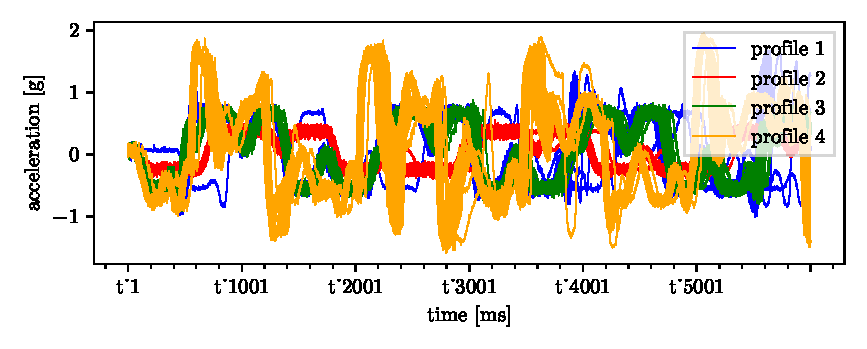
\includegraphics{images/LinearMotor/Timeseries.pdf}
    \caption{Timeseries of the training set}
    \label{fig:axis_timeseries}
\end{figure}


\begin{figure}
    \centering
    \includegraphics[width=\textwidth]{images/LinearMotor/Features.pdf}
    \caption{features of the training set}
    \label{fig:axis_features}
\end{figure}

\begin{figure}
    \centering
    \includegraphics{images/LinearMotor/Scatter.pdf}
    \caption{Visualization of the separation between profiles in the feature space}
    \label{fig:axis_scatter}
\end{figure}


\subsection{Testing on a known profile}
The microcontroller is then set in \emph{evaluate} mode and the \gls{nd} is performed on a loop that repeats the movement of profile 2. The result of this first model (Model 1) is shown in \autoref{fig:axis_testing}. We can see that the model immediately falsely detects a novelty, despite profile 2 being part of the training set. The figure also shows a clearer view of the evolution of the novelty score, obtained by applying a moving average filter on the last 5 values of the novelty metric.

Let's investigate why this model gives almost all false positive results. Analyzing the features of the training set (\autoref{fig:axis_features}), we can see that the first features, up to $\approx 12$, are grouped by profile, but most of the remaining features are not, this arises the suspect that these features may not be significative of the movement, but maybe just representing noise. This is likely also because the necessary standardization procedure ensures that each feature will have unitary standard deviation, regardless of the magnitude of the feature itself \gls{wrt} the others. This may cause \quoted{noise} features to be amplified in the model. Moreover, it's clear that, being most of the features not significant, the model is not able to distinguish between the profiles.

In \autoref{fig:axis_scatter}, a better visualization of the problem is presented. Features 5 and 6 are significative of the specific movement as we can see in the scatter plot, because the data points are grouped by profile. Features 25 and 26, instead, are not significative, as the data points are not grouped by profile.



\begin{figure}
    \centering
    \includegraphics[angle=-90,origin=c]{images/LinearMotor/Testing.pdf}
    \caption{Novelty detection on profile 2.}
    \label{fig:axis_testing}
\end{figure}
\clearpage


\subsection{Feature scaling}
To address the problem of the non-significative features, a feature scaling method is proposed. The idea is to scale the features in such a way that the most significant features will have a higher weight in the model. To do that, a naive approach could be to visually select the important features (by eye it's evident that are the first few) and apply a small scaling factor to the others. 

This approach goes against the principle of the framework being fully automatic to train. To address this problem, an unsupervised and automatic method is proposed. The idea is to scale the features in such a way that the most significant features will have a higher weight in the model. To do that, it's possible to exploit the fact that, at this point, the K-means model is already trained and the training procedure provided labels for the dataset. It's now possible to apply a \emph{supervised} \gls{ml} algorithm in a way that is transparent to the user, so the whole procedure remains \emph{unsupervised}.

The framework is then extended to include the possibility of applying feature scaling. The two possibilities are to use the Random Forest classifier or the SelectKBest algorithm to provide the weights. Since this scaling will affect also future snapshots, a new train of the \gls{mla} is necessary. The new model is then trained with the same training set but with the scaled features. This approach is illustrated in \autoref{fig:scalingprocedure}.

\begin{figure}[h!]
    \centering
    \includegraphics{images/LinearMotor/Feat_scaling.pdf}
    \caption{Feature scaling procedure.}
    \label{fig:scalingprocedure}
\end{figure}

This scaling technique is used with several configurations for both scaling the feature and reducing the number of features, by discarding the unnecessary ones. The settings of each tuned model are resumed in \autoref{tab:axis_models}. These models are described later in this section.

\begin{table}
    \centering
    \caption{Tuned embedded models parameters}
    \label{tab:axis_models}
    \resizebox{\linewidth}{!}{%
    \begin{tabular}{ccccccccc} 
    \toprule
    \multirow{2}{*}{\textbf{Model}} & \multicolumn{2}{c}{\textbf{Feature Scaling}} & \multirow{2}{*}{\begin{tabular}[c]{@{}c@{}}\textbf{Feature}\\\textbf{Subset}\end{tabular}} & \multicolumn{4}{c}{\begin{tabular}[c]{@{}c@{}}\textbf{Training Snapshots}\\(per each profile)\\\end{tabular}} & \multirow{2}{*}{\begin{tabular}[c]{@{}c@{}}\textbf{N of}\\\textbf{clusters}\end{tabular}} \\
     & SelectKBest & Random Forest &  & 1 & 2 & 3 & 4 &  \\ 
    \hline
    Model 1 &  &  &  & 100 & 100 & 100 & 100 & 5 \\
    Model 2 &  & \checkmark &  & 100 & 100 & 100 & 100 & 3 \\
    Model 3 & \checkmark &  &  & 100 & 100 & 100 & 100 & 3 \\
    Model 4 &  & \checkmark &  & 100 & 200 & 100 & 100 & 5 \\
    Model 5 &  & \checkmark & \checkmark & 100 & 100 & 100 & 100 & 6 \\
    \bottomrule
    \end{tabular}
    }
    \end{table}

\subsubsection{Random Forest}
The Random Forest classification algorithm gives a measure of the importance of each feature, and this measure can be used to scale the features. The \gls{rf} algorithm is trained on the training set, with the labels provided by the K-means model. 

The feature importance is based on the idea that the Gini impurity is reduced at a split in each decision tree of the forest. The more the impurity is reduced, the more important the feature used for that split is \cite{RF_featimportance}. This concept, averaged over all splits of all the trees, gives a measure of the importance of each feature.

For our purpose, the importance is then normalized to have a maximum value of~1, so the most important feature will remain unscaled.

\subsubsection{SelectKBest}
Another tool for analyzing the importance of features is the SelectKBest algorithm. It is available in the \texttt{scikit-learn} library and is used to select the $k$ most important features or, alternatively, to output a score for each feature, based on \gls{anova} statistics.

\subsubsection{Results}
At this point, both the training of the \gls{rf} and SelectKBest is performed. The weights obtained with both methods are shown in \autoref{fig:axis_weights}. The two methods gave very similar results. Now it is possible to train the \gls{mla} with the scaled features, Model 2 and Model 3 are trained with the \gls{rf} and SelectKBest weights, respectively. Both models perform better than the original model because they give a smaller novelty score for the testing set. However, the problem of eliminating the false positive results is not yet solved, because the novelty score is still greater than zero.

\begin{figure}
    \centering
    \includegraphics[width=\textwidth]{images/LinearMotor/Feat_weights.pdf}
    \caption{Feature weights obtained with the \gls{rf} and SelectKBest algorithms}
    \label{fig:axis_weights}
\end{figure}

To further refine the model, a fourth version is provided, this time extending the training set to include the first 100 samples of this testing set. So the Model 4 will be trained on a total of 200 snapshots for profile 2. In the \autoref{fig:axis_testing}, of course, the novelty score is always negative for the first 100 samples, because they are part of the training set. Then, the novelty score becomes positive only in isolated cases, and even then it remains quite low. In this scenario, a novelty threshold of 20\% is enough to run all the dataset without any false positive result, even without the activation of the outlier filter.

\subsection{Testing the \gls{nd}}
The previous experiment was done to test the capability of the framework to identify a known profile. Now the framework is tested to identify a profile that is not part of the training set, so it should trigger a \gls{nd} event. The test consists of actuating the axis alternating between unknown profiles and known profiles (10 snapshots each repetition). For reference, also Model 1, Model 2, and Model 3 are used, even if they were discarded in the previous section. 

The results are shown in \autoref{fig:axis_testing2}. Model 4 performs poorly because, even if it avoids completely giving false positive results, it gives a lot of false negative results. Unknown profiles are not detected as novelties, or they are detected only in isolated cases, with a very low novelty score that is not enough to trigger the \gls{nd} event, considering the threshold discussed in the previous section.

\begin{figure}
    \centering
    \includegraphics{images/LinearMotor/Testing2.pdf}
    \caption{Novelty detection on known and unknown profiles}
    \label{fig:axis_testing2}
\end{figure}
}